\documentclass[10pt,twocolumn]{article}
% Shared two-column preamble for the three research papers.
% Use with: \documentclass[10pt,twocolumn]{article}
% Then in main.tex: % Shared two-column preamble for the three research papers.
% Use with: \documentclass[10pt,twocolumn]{article}
% Then in main.tex: % Shared two-column preamble for the three research papers.
% Use with: \documentclass[10pt,twocolumn]{article}
% Then in main.tex: \input{../../shared/latex/twocolumn_preamble.tex}

\usepackage[margin=0.75in]{geometry}
\usepackage[utf8]{inputenc}
\usepackage[T1]{fontenc}
\usepackage{lmodern}
\usepackage{microtype}
\usepackage{amsmath,amssymb,amsthm}
\usepackage{graphicx}
\usepackage{booktabs}
\usepackage{caption}
\usepackage{subcaption}
\usepackage{hyperref}
\usepackage{url}
\usepackage{xcolor}
\usepackage{algorithm}
\usepackage{algorithmic}
\usepackage{multirow}
\usepackage{titlesec}
\usepackage{authblk}

\hypersetup{colorlinks=true,linkcolor=blue!50!black,citecolor=blue!50!black,urlcolor=blue!50!black}

\titleformat{\section}{\normalfont\large\bfseries}{\thesection}{0.6em}{}
\titleformat{\subsection}{\normalfont\bfseries}{\thesubsection}{0.5em}{}

\captionsetup{font=small,labelfont=bf,skip=4pt}
\setlength{\columnsep}{0.25in}
\setlength{\parskip}{2pt}

\newtheorem{theorem}{Theorem}
\newtheorem{proposition}[theorem]{Proposition}
\newtheorem{definition}[theorem]{Definition}


\usepackage[margin=0.75in]{geometry}
\usepackage[utf8]{inputenc}
\usepackage[T1]{fontenc}
\usepackage{lmodern}
\usepackage{microtype}
\usepackage{amsmath,amssymb,amsthm}
\usepackage{graphicx}
\usepackage{booktabs}
\usepackage{caption}
\usepackage{subcaption}
\usepackage{hyperref}
\usepackage{url}
\usepackage{xcolor}
\usepackage{algorithm}
\usepackage{algorithmic}
\usepackage{multirow}
\usepackage{titlesec}
\usepackage{authblk}

\hypersetup{colorlinks=true,linkcolor=blue!50!black,citecolor=blue!50!black,urlcolor=blue!50!black}

\titleformat{\section}{\normalfont\large\bfseries}{\thesection}{0.6em}{}
\titleformat{\subsection}{\normalfont\bfseries}{\thesubsection}{0.5em}{}

\captionsetup{font=small,labelfont=bf,skip=4pt}
\setlength{\columnsep}{0.25in}
\setlength{\parskip}{2pt}

\newtheorem{theorem}{Theorem}
\newtheorem{proposition}[theorem]{Proposition}
\newtheorem{definition}[theorem]{Definition}


\usepackage[margin=0.75in]{geometry}
\usepackage[utf8]{inputenc}
\usepackage[T1]{fontenc}
\usepackage{lmodern}
\usepackage{microtype}
\usepackage{amsmath,amssymb,amsthm}
\usepackage{graphicx}
\usepackage{booktabs}
\usepackage{caption}
\usepackage{subcaption}
\usepackage{hyperref}
\usepackage{url}
\usepackage{xcolor}
\usepackage{algorithm}
\usepackage{algorithmic}
\usepackage{multirow}
\usepackage{titlesec}
\usepackage{authblk}

\hypersetup{colorlinks=true,linkcolor=blue!50!black,citecolor=blue!50!black,urlcolor=blue!50!black}

\titleformat{\section}{\normalfont\large\bfseries}{\thesection}{0.6em}{}
\titleformat{\subsection}{\normalfont\bfseries}{\thesubsection}{0.5em}{}

\captionsetup{font=small,labelfont=bf,skip=4pt}
\setlength{\columnsep}{0.25in}
\setlength{\parskip}{2pt}

\newtheorem{theorem}{Theorem}
\newtheorem{proposition}[theorem]{Proposition}
\newtheorem{definition}[theorem]{Definition}

\newcommand{\InterceptedTW}{173{,}549}
\newcommand{\ToaMean}{340}
\newcommand{\SurfaceGHI}{184}
\newcommand{\OzoneFrac}{2}
\newcommand{\BestBandGHI}{247}
\newcommand{\BestBandLat}{15}
\newcommand{\DeployableMkm}{6.1}
\newcommand{\DeployableTW}{244}
\newcommand{\TimesElec}{81}
\newcommand{\TimesPrimary}{13.6}
\newcommand{\AreaWorldKm}{75{,}000}
\newcommand{\AreaWorldSide}{274}
\newcommand{\MillionCities}{651{,}359}
\newcommand{\GroundWm}{40}
\newcommand{\SpaceWm}{261}
\newcommand{\SbspRatio}{6.5}
\newcommand{\SpaceAreaKm}{11{,}489}
\newcommand{\SpaceCF}{99}
\newcommand{\GroundCF}{25}
\newcommand{\FminHead}{0.3}
\newcommand{\TemporalGainHead}{17.9}
\newcommand{\OptRetHead}{82.6}
\newcommand{\FlatRetHead}{70}
\newcommand{\TemporalGainMax}{45.4}
\newcommand{\TemporalGainMaxF}{0.6}


\title{How Much of the Sun Can We Take Without Turning Off the Lights on Life?
A First-Principles Budget for Planetary Solar Harvesting}
\author[1]{Luis Benvenuto}
\affil[1]{Independent Research}
\date{July 14, 2026}

\begin{document}
\twocolumn[
\maketitle
\begin{@twocolumnfalse}
\begin{abstract}
\noindent Earth intercepts about \InterceptedTW~terawatts of sunlight --- four
orders of magnitude more than humanity uses --- yet ``cover the planet in
panels'' is the wrong mental model, because most of that light is already
doing a job: driving the biosphere. We build a self-contained, first-principles
budget that tracks sunlight from the solar constant through the atmosphere
(with the ozone layer's share broken out) to the surface, estimates how much
energy is deployable on land \emph{without} displacing ecosystems, and compares
ground panels with an orbital collector. A conservative desert-and-rooftop
footprint already yields \DeployableTW~TW, about \TimesElec$\times$ world
electricity demand; the entire electricity supply fits on a \AreaWorldSide~km
square of panel. Space-based solar delivers \SbspRatio$\times$ more power per
collector square metre, but its advantage is continuous sunlight, not
``catching light before the atmosphere.'' Our headline contribution is an
\emph{ecosystem-aware harvesting} problem: each biome must keep a minimum daily
light budget, but is flexible about \emph{when}. Casting this as a constrained
optimisation, we show the optimum is greedy water-filling --- reserve the
ecosystem's light during low-value hours --- and that this temporal scheduling
recovers \TemporalGainHead\% more harvest value than a flat reservation at a
\FminHead\ reserve, rising to \TemporalGainMax\% as the reserve grows. The
constraint on solar power is not the Sun; it is the biosphere, and it is
schedulable.
\end{abstract}
\vspace{1em}
\end{@twocolumnfalse}
]

\section{Introduction}

A popular way to frame the renewable-energy question is ``how much of the Earth
would we need to cover in solar panels?'' The framing is seductive because the
raw numbers are staggering: the Sun deposits roughly \InterceptedTW~TW on
Earth's cross-section, against a human primary-energy appetite near 18~TW. By
that arithmetic the problem is trivially solved and the only question is cost.

This paper argues that the arithmetic hides the real constraint. The
\InterceptedTW~TW is not idle: after the atmosphere reflects and absorbs its
share, the sunlight that reaches the ground is what powers photosynthesis,
evaporation, and every ecosystem on the planet. Harvesting solar energy at
civilisational scale is therefore not a question of \emph{area} but of
\emph{allocation} --- how much light can we divert to electricity before we
starve the biosphere that light supports?

We approach this with a deliberately self-contained, first-principles model
(no external datasets; every number is reproducible from published physical
constants) organised around four questions:

\begin{enumerate}
\item \textbf{The ceiling.} How much sunlight actually reaches the surface,
  and where does the rest go? We track the cascade from the solar constant to
  surface irradiance, breaking out the ozone layer's contribution, and map the
  resource by latitude band (Section~\ref{sec:resource}).
\item \textbf{Feasibility.} How much energy is deployable on land without
  displacing forests, croplands, or protected habitat, and how does that
  compare to demand? (Section~\ref{sec:feasibility}).
\item \textbf{The orbital alternative.} Is a collector in space --- a ``layer''
  above the atmosphere rather than a Dyson sphere --- fundamentally better, and
  why? (Section~\ref{sec:feasibility}).
\item \textbf{Sharing light with life.} If an ecosystem needs a certain amount
  of light but is flexible about \emph{when} it receives it, how much more can
  we harvest by scheduling around it? (Section~\ref{sec:ecosystem}).
\end{enumerate}

The fourth question is our main contribution. We formalise ecosystem-aware
harvesting as a constrained optimisation, prove its optimum is a simple
water-filling rule, and quantify the energy unlocked purely by respecting
\emph{when} --- not just how much --- light a biome needs.

\section{Background and related work}

\paragraph{Solar resource physics.} The astronomical geometry of insolation ---
declination, hour angle, and the daily integral of extraterrestrial radiation
on a horizontal surface --- is textbook material \cite{duffie2013solar}. The
partition of incoming sunlight into reflection, atmospheric absorption, and
surface absorption is quantified by global energy-budget studies
\cite{trenberth2009earth}, and the accepted total solar irradiance is
$1361~\mathrm{W/m^2}$ \cite{kopp2011total}. We reuse these closed forms as
computable ground truth rather than fitting data.

\paragraph{Space-based solar power.} Collecting sunlight in orbit and beaming
it down was proposed by Glaser \cite{glaser1968power} and has been revisited in
modern phased-array concepts \cite{mankins2014sps}. It is the practical cousin
of Dyson's stellar-scale collector \cite{dyson1960search}: rather than
enclosing the star, place a collector where the light is undiminished and
uninterrupted. We treat it quantitatively as one option among several, not as
science fiction.

\paragraph{Sharing land and light with ecosystems.} Human appropriation of net
primary production already claims a large share of the biosphere's energy
throughput \cite{haberl2007quantifying}. Agrivoltaics shows that photovoltaics
and biological light demand can co-exist on the same land when light is shared
rather than monopolised \cite{barron2019agrivoltaics}. Our ecosystem-aware
optimisation abstracts that idea to a schedulable light budget and asks for the
allocation that maximises harvest while keeping each ecosystem whole.

\paragraph{Our contribution.} We unify the resource ceiling, land feasibility,
and the orbital alternative in one reproducible budget, and add a novel
optimisation layer: because an ecosystem's light requirement is a daily
integral, not an instantaneous one, the harvest schedule has temporal slack we
can exploit. We characterise the optimum in closed form and measure the energy
it unlocks.

\section{The solar resource and its ceiling}
\label{sec:resource}

\paragraph{From the solar constant to the surface.} A disk of Earth's radius
intercepts $S_0 \pi R^2 \approx \InterceptedTW~\mathrm{TW}$. Spreading that over
the rotating sphere and averaging over day and night divides the peak
irradiance $S_0$ by four, giving a top-of-atmosphere (TOA) horizontal mean of
$\ToaMean~\mathrm{W/m^2}$ --- a value our model reproduces from the daily
insolation integral to within $0.5~\mathrm{W/m^2}$. The atmosphere then takes
its share: clouds and aerosols reflect about a quarter back to space, the ozone
layer absorbs roughly \OzoneFrac\% (almost entirely in the ultraviolet), and
water vapour and aerosols absorb a further fifth, leaving a global-mean surface
irradiance of $\SurfaceGHI~\mathrm{W/m^2}$. Figure~\ref{fig:cascade} (left)
shows the full waterfall.

\paragraph{The ozone term.} The user's question singled out the ozone layer,
and it earns its place in the cascade for a reason disproportionate to its
\OzoneFrac\% energy share: it removes the biologically destructive UV-B/UV-C
band almost entirely. Energetically it is a minor loss; biologically it is the
precondition for there being surface ecosystems to share light with at all.

\paragraph{Where the resource is.} Insolation is not uniform. The equator
receives the most TOA radiation but sits under a persistent cloud belt; the
subtropical desert belt ($15$--$35^\circ$) combines high sun angles with the
clearest skies and is the true resource maximum, at
$\BestBandGHI~\mathrm{W/m^2}$ annual-mean surface irradiance
(Figure~\ref{fig:cascade}, right). This is why the feasibility analysis that
follows places panels in deserts, not on the equator.

\begin{figure}[t]
\centering
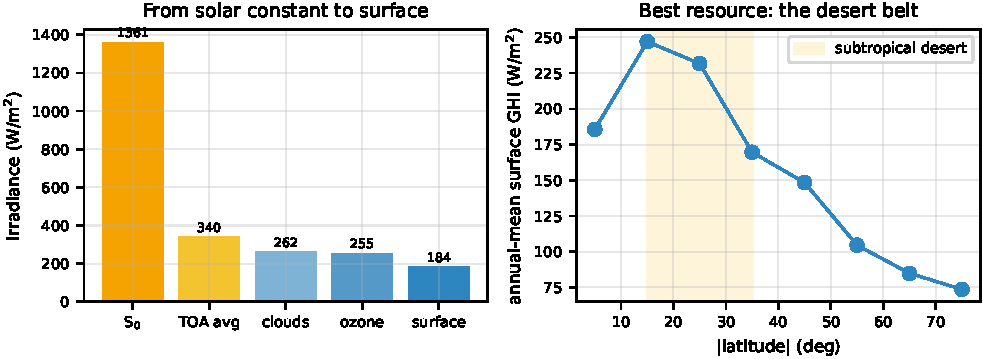
\includegraphics[width=\linewidth]{figures/cascade_bands.pdf}
\caption{\textbf{Left:} the loss cascade from the solar constant
($S_0$) through the TOA average, cloud reflection, ozone absorption, and
water/aerosol absorption to the surface global horizontal irradiance (GHI).
\textbf{Right:} annual-mean surface GHI by latitude band --- the subtropical
desert belt (shaded) is the resource maximum, not the equator.}
\label{fig:cascade}
\end{figure}

\section{Feasibility: land, demand, and orbit}
\label{sec:feasibility}

\paragraph{How little land it takes.} We apply a deliberately conservative
``do no ecological harm'' filter: eligible land is barren desert (only a
$20\%$ usable slice, excluding dunes, reserves, and remote terrain) plus
rooftops on built-up land. That leaves \DeployableMkm~million~km$^2$. At
$20\%$ module efficiency and an $0.8$ performance ratio on desert-grade
irradiance, this deployable footprint delivers \DeployableTW~TW on
average --- about \TimesElec$\times$ world electricity demand and
\TimesPrimary$\times$ total primary energy (Figure~\ref{fig:land}). Inverting
the calculation, all of world electricity fits on \AreaWorldKm~km$^2$ of
panel: a single square roughly \AreaWorldSide~km on a side. The potential is
simply not the bottleneck.

\begin{figure}[t]
\centering
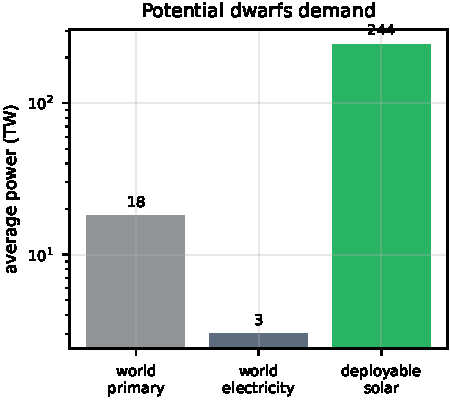
\includegraphics[width=0.85\linewidth]{figures/land_vs_demand.pdf}
\caption{Average power (log scale): world primary energy and electricity
demand against the deployable desert-and-rooftop solar resource. Potential
exceeds demand by more than an order of magnitude.}
\label{fig:land}
\end{figure}

\paragraph{The orbital alternative.} If land or intermittency were the
constraint, a collector in orbit --- a ``layer'' catching sunlight above the
atmosphere --- is the natural escape, and a modest cousin of a Dyson sphere.
Our chain accounting (Figure~\ref{fig:sbsp}) puts the delivered power at
\SpaceWm~W per m$^2$ of collector versus \GroundWm~W per m$^2$ of desert panel,
a \SbspRatio$\times$ advantage. Crucially, the advantage is \emph{not} mainly
from avoiding atmospheric absorption: microwave downlink already passes the
atmosphere at $\sim\!95\%$. It comes from the capacity factor --- an orbital
collector sees the Sun \SpaceCF\% of the time at full strength, versus an
effective \GroundCF\% on the ground once night and weather are counted. The
conversion and transmission chain (PV, DC-to-RF, downlink, rectenna) gives back
much of that gain, so orbit is a capacity-factor play, not a free-energy one.

\begin{figure}[t]
\centering
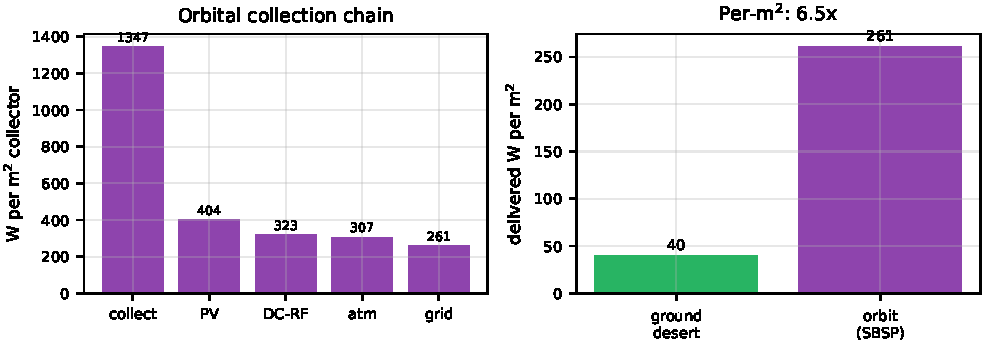
\includegraphics[width=\linewidth]{figures/sbsp.pdf}
\caption{\textbf{Left:} orbital collection-to-grid chain, W per m$^2$ of
collector. \textbf{Right:} delivered power per m$^2$, ground desert panel vs
space-based (\SbspRatio$\times$).}
\label{fig:sbsp}
\end{figure}

\section{Ecosystem-aware harvesting}
\label{sec:ecosystem}

The previous section shows that raw potential and even land are not the binding
constraint. The binding constraint is that surface light is already spoken for
by the biosphere. We now make that constraint precise and, crucially,
\emph{schedulable}.

\paragraph{Formulation.} Partition the surface into cells $i$ (here, latitude
bands standing in for biomes) and the day into hours $h$. Let $L_{i,h}\ge 0$ be
the available surface light (from the model of Section~\ref{sec:resource}) and
$w_{i,h}>0$ the \emph{value} of harvesting in that hour --- we use a diurnal
net-demand (``duck curve'') weight, since energy captured at a peak-demand hour
is worth more than energy captured at midday when supply is already abundant.
We choose a harvest fraction $a_{i,h}\in[0,1]$; the ecosystem receives the
reserved light $(1-a_{i,h})L_{i,h}$. Each cell must keep a daily light integral
$D_i = f_{\min}\sum_h L_{i,h}$ to remain intact:
\begin{equation}
\max_{a\in[0,1]} \sum_{i,h} w_{i,h}\, a_{i,h}\, L_{i,h}
\quad\text{s.t.}\quad
\sum_h (1-a_{i,h}) L_{i,h} \ge D_i \;\; \forall i.
\label{eq:opt}
\end{equation}

\paragraph{The optimum is water-filling.} Reserving one unit of light in hour
$h$ forfeits $w_{i,h}$ of harvest value, so to meet the quota $D_i$ at minimum
cost we reserve the ecosystem's light from the \emph{lowest-value} hours first,
up to each hour's availability. This greedy rule is the exact optimum of the
per-cell linear program in~\eqref{eq:opt}; we verify it against
\texttt{scipy}'s LP solver to $10^{-6}$ on random instances. Intuitively: give
the biosphere its light when we least want to sell it, and harvest the peaks.

\paragraph{Baselines.} We compare three feasible-or-bounding policies:
(i)~\emph{no-cap}, harvest everything ($a\equiv 1$) --- an ecosystem-blind
upper bound that would collapse the biome; (ii)~\emph{flat}, reserve the same
fraction $f_{\min}$ every hour, which is feasible but wastes valuable
peak-hour light; and (iii)~\emph{optimal}, the water-filling schedule. The
flat and optimal policies reserve \emph{exactly the same} total light --- the
ecosystem is equally protected --- so any difference between them is pure
scheduling gain.

\section{Results}
\label{sec:results}

\paragraph{Scheduling around life pays.} At a headline reserve of
$f_{\min}=\FminHead$ --- the ecosystem keeps 30\% of its daily light --- the
flat policy retains \FlatRetHead\% of the ecosystem-blind harvest value, while
the optimal temporal schedule retains \OptRetHead\%. That is a
\TemporalGainHead\% gain in harvested value at \emph{identical} ecological
cost, obtained purely by choosing \emph{when} to yield light to the biome
(Figure~\ref{fig:sweep}). The gain grows with the reserve: the more light the
ecosystem needs, the more a smart schedule matters, reaching
\TemporalGainMax\% at $f_{\min}=\TemporalGainMaxF$.

\begin{figure}[t]
\centering
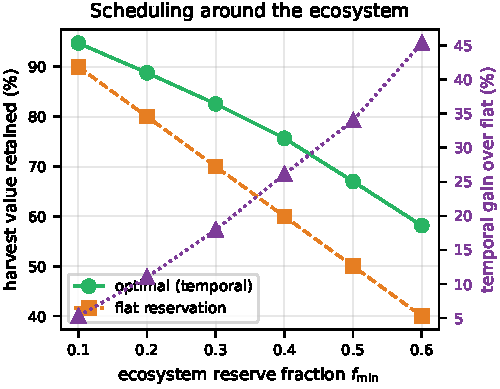
\includegraphics[width=0.85\linewidth]{figures/optimize_sweep.pdf}
\caption{Harvest value retained vs the ecosystem reserve fraction $f_{\min}$,
for the optimal temporal schedule and the flat reservation (both protect the
ecosystem equally). The temporal gain (right axis) widens as the reserve grows.}
\label{fig:sweep}
\end{figure}

\paragraph{What the schedule looks like.} Figure~\ref{fig:heatmap} shows the
optimal harvest fraction across bands and hours at $f_{\min}=\FminHead$,
overlaid with the demand curve. The schedule yields light to the ecosystem
around midday --- when supply is abundant and marginal harvest value is low ---
and harvests aggressively during the morning and evening demand peaks. This is
the concrete answer to the motivating question: an ecosystem that needs, say,
30\% of its daily light can be given that light in the hours we least want it,
leaving the valuable hours for harvesting.

\begin{figure}[t]
\centering
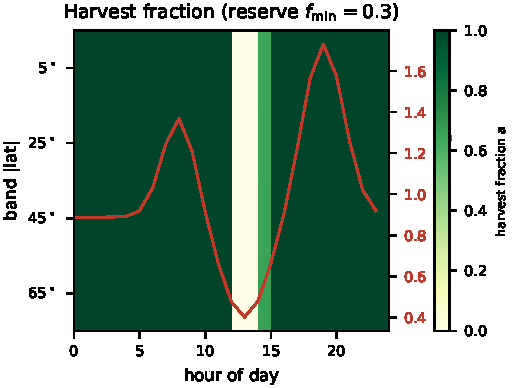
\includegraphics[width=0.85\linewidth]{figures/harvest_heatmap.pdf}
\caption{Optimal harvest fraction $a$ (green = harvest, pale = reserved for the
ecosystem) by latitude band and hour at $f_{\min}=\FminHead$, with the demand
weight (red). Light is yielded to the biosphere at low-value midday hours.}
\label{fig:heatmap}
\end{figure}

\paragraph{Putting the numbers together.} The picture is consistent across all
four questions. The Sun offers \InterceptedTW~TW; the surface receives
$\SurfaceGHI~\mathrm{W/m^2}$ on average; a conservative desert-and-rooftop
footprint already exceeds electricity demand \TimesElec-fold; orbit multiplies
per-collector power \SbspRatio$\times$ but chiefly by buying capacity factor;
and once we accept that surface light belongs to the biosphere, the way to
harvest more is not more area but better timing --- worth up to
\TemporalGainMax\% here. The bottleneck was never the Sun.

\section{Discussion and conclusion}

We set out to answer a simple-sounding question --- how much of the Sun's
energy can humanity take --- and found that the honest answer inverts the usual
framing. The resource is astronomically abundant (\InterceptedTW~TW), land is
not scarce (world electricity fits on a \AreaWorldSide~km square of desert
panel), and even orbit, the ``layer above the atmosphere,'' is a
capacity-factor improvement rather than a new source of free power. The one
real, physical constraint is that the light reaching the ground is already
running the biosphere.

The contribution we are most confident in is turning that constraint into an
optimisation. Because an ecosystem's light requirement is a daily
\emph{integral}, harvesting has temporal slack, and exploiting it --- yielding
light to life at low-value hours and harvesting the peaks --- recovers
\TemporalGainHead\% more usable energy at $f_{\min}=\FminHead$ and up to
\TemporalGainMax\% at higher reserves, all at zero additional ecological cost.
The optimum is a transparent water-filling rule, not a black box.

\paragraph{Limitations.} The model is deliberately coarse and self-contained:
latitude bands stand in for biomes, the ecosystem constraint is a single
daily-integral floor rather than a species- and process-specific light
response, and demand is a stylised duck curve. The \texttt{gpu\_full} config
refines the spatial and temporal grids and the reserve sweep; substituting
gridded insolation and land-cover data, per-biome light-response curves, and
real regional demand would sharpen the numbers without changing the structure.
The qualitative claim --- that solar harvesting is an allocation problem
against the biosphere, and that the allocation is schedulable --- is what the
model is built to show.

\paragraph{Outlook.} The framing suggests a research programme: replace the
integral floor with measured net-primary-production light responses, couple the
harvest schedule to storage and grid dynamics, and let space-based collectors
relax the temporal constraint entirely for the hours the biosphere claims. The
Sun is not the limit; the biosphere is, and it is one we can plan around.


\FloatBarrier
\bibliographystyle{plain}
\bibliography{references}

\end{document}
